\documentclass[a4paper]{article}

\usepackage{cmap}
\usepackage[T2A]{fontenc}
\usepackage[utf8]{inputenc}
\usepackage[english,russian]{babel}
\usepackage{amsmath,amsfonts,amssymb,amsthm,mathtools}

\usepackage{amsmath}

\usepackage{amsmath}
\usepackage{tikz}
\usepackage{mathdots}
\usepackage{yhmath}
\usepackage{cancel}
\usepackage{color}
\usepackage{siunitx}
\usepackage{array}
\usepackage{multirow}
\usepackage{amssymb}
\usepackage{gensymb}
\usepackage{tabularx}
\usepackage{booktabs}
\usepackage{amsmath, amsfonts}
\usepackage{mathtext}
\usepackage{dsfont}
\usepackage{xcolor}
\usepackage{hyperref}
\usetikzlibrary{fadings}
\usetikzlibrary{patterns}
\usetikzlibrary{shadows.blur}
\usepackage{graphicx}
\graphicspath{{pictures/}}

\title{Текст к слайдам}
\author{Гусев Владислав БПМИ187}
\date{\today}

\begin{document}

\maketitle

\section*{1 Слайд: общими словами про модель и ученых:}
Модель ценообразования опционов была впервые представлена общественности в 1973 году двумя учеными: Фишером Блэком (Fisher Black) и Майраном Шоулзом (Myron Scholes). В настоящее время она широко известна как «модель Блэка-Шоулза» (англ. Black-Scholes Option Pricing Model). Авторами была предложена математическая модель описывающая рынок финансовых деривативов (в нашем случае только опционы). Практическим результатом модели стала формула Блэка-Шоулза, которая позволила рассчитать цену опциона колл европейского типа. Ее появление привело к буму торговли опционами, а сама она получила широкое применение среди участников рынка.

\section*{2 Слайд: Что такое опционы и их характеристики:}
Опцион — это договор, по которому покупатель опциона получает право купить/продать какой-либо актив (товар, ценная бумага, валюта и др.) в определенный момент времени по заранее обусловленной цене. 

При этом Обязанность по исполнению опциона ложится на его продавца, который может выступать как покупателем (put option), так и продавцом (call option) базового актива. В то время как покупатель, имея опцион, имеет право не использовать его.

По времени исполнения выделяются следующие типы инструмента: \\
- европейский — может быть исполнен только в последний день срока; \\
- американский — реализуется в любое время до окончания контракта; \\
- квазиамериканский, который погашается владельцем в определенные временные промежутки (договор предусматривает один или более отрезков). 

Также опционы делятся на два главных класса: CALL и PUT:
Опцион колл дает его покупателю право на покупку базового актива по фиксированной цене в определенное время. Соответственно, опцион пут дает право на продажу актива по заданной цене в заданное время.

Также стоит отметить, что приобретая опцион, покупатель платит продавцу премию — денежное вознаграждение за право покупки (продажи) базового актива по опционному договору -- и именно эту стоимость рассчитывает «модель Блэка-Шоулза»


\section*{3 Слайд: вывод модели Блэка-Шоулза}
Уравнение Блэка-Шоулза является дифференциальным уравнением в частных производных, которое описывает цену опциона колл во времени.

Вывод модели основывается на концепции безрискового хеджирования. Покупая акции и одновременно покупая опционы PUT на эти акции, инвестор может конструировать безрисковую позицию, где прибыли по акциям будут точно компенсировать убытки по опционам, и наоборот.

Безрисковая хеджированная позиция должна приносить доход по ставке, равной безрисковой процентной ставке, в противном случае существовала бы возможность извлечения арбитражной прибыли и инвесторы, пытаясь получить преимущества от этой возможности, приводили бы цену опциона к равновесному уровню, который определяется моделью.

\subsubsection*{Вывод формулы:}
Предполагается, что стоимость опциона зависит только от цены акции и времени, а также переменных, которые считаются константами. \\
$w(x, t)$ -- значение опциона, как функция цены акции $x$ и времени $t$. Поэтому количество опционов, которые должны быть проданы по отношению к купленной акции равно: $\dfrac{1}{(w(x,t)'_x)}$. (если цена акции изменить на $\Delta x \Rightarrow$  цена опциона измениться на $w(x,t)’_x \cdot \Delta x$, а количество опционов измениться на $\Delta x$. Что показывает компенсацию изменения цены стоимостью опционов.

Так как $x$ и $t$ постоянно изменяются, то поддержание хеджируемой позиции должно быть непрерывным.


В целом, если на одну акцию имеет $\dfrac{1}{w(x, t)'_x}$ опционов, то количество капитала в позе: $x - \dfrac{w}{w(x, t)'_x}$.

Изменение капитала в хеджируемой за короткий интервал $\Delta t: \Delta x - \dfrac{\Delta w}{w(x, t)’_x}$

Так как позиция изменяется непрерывно, то расчитать $\Delta w = w(x + \Delta x, t + \Delta t) - w(x, t)$:
\[\Delta w = w'_x \Delta x + \frac{1}{2} (w'_x)'_x v^2 x^2 \Delta t + w'_t \delta t\]
где $v^2$ -- коэффицент доходности акций.

Подставим полученное выражение в формулу изменения капитала за $\Delta t$ и получим:
\[- \left(\dfrac{1}{2} (w'_x)'_x v^2 x^2 + w'_t \right) \dfrac{\Delta t}{w'_x}\]
Так как доходность капитала в хеджирумой позиции определена, то возвратный коэффицент будет равен $r \Delta t$, чтобы выполнялось условие доходности только по процентной ставке r. Следовательно изменение капитала должно быть равно значиню капитала, умноженного на $r \Delta t$:
\[- \left(\dfrac{1}{2} (w'_x)'_x v^2 x^2 + w'_t \right) \dfrac{\Delta t}{w'_x} = (x - \dfrac{w}{w'_x}) \cdot r \Delta t\]
делим на $\Delta t $ с обеих сторон и получаем дифференцальное уравнение для стоимости опциона:
\[w'_t = rw - rxw'_x - \dfrac{1}{2} v^2 x^2 (w'_x)'_x\]
Берем $t^*$ -- дата экспирации опциона, $c$ -- цена исполнения опциона, тогда знаем такие ограничения:

\begin{equation*}
    \begin{cases}
        w(x, t^*) = x - c, &x \geq c\\
        0, &x < c \\
    \end{cases}
\end{equation*}

Далее делается замена: \\
\[ w(x,t) = e^{r (t - t^*)} y \left[ \left(\frac{2}{v^2} \right) \left( r - \dfrac{1}{2} v^2\right) \left[ ln(\dfrac{x}{c}) - \left( r - \dfrac{1}{2} v^2 \right) (t - t^*) \right], - \left( \dfrac{2}{v^2} \right) \left( r - \dfrac{1}{2} v^2 \right)^2 (t - t^*) \right] \]
где $y$ -- функия от двух переменных. \\
И после замены дифференцальное уравнение будет выглядеть так:
\[y'_t = (y'_x)'_x\]
А ограничения будут выглядеть так:
\begin{equation*}
    \begin{cases}
        y(u, 0) = 0, &u < 0\\
        c \left[ e^{u \left( \dfrac{1}{2} v^2\right) / \left( r - \dfrac{1}{2} v^2\right)} - 1 \right], &u \geq 0 \\
    \end{cases}
\end{equation*}
Данное уравнение является физическим уравнением теплопередачи. Его решение:
\[y(u, s) = \dfrac{1}{\sqrt{2 \pi}} \int_{\dfrac{-u}{\sqrt{2s}}}^{\infty} \left( c \left[ e^{(u + q \sqrt{2s}) \left( \dfrac{1}{2} v^2 \right)} / \left( r - \dfrac{1}{2} v^2\right) - 1 \right] e^{\dfrac{-q^2}{2}} dq \right) \] 
производим обратную замену, упрощаем и получаем:
\[ w(x, t) = x N(d_1) - ce^{r (t - t^*)} N(d_2) \]
\[ d_1 = \dfrac{ln \left(\dfrac{x}{c} \right) + \left( r + \dfrac{1}{2} v^2 \right) (t* - t)}{v \sqrt{t^* - t}}\]
\[ d_2 = \dfrac{ln \left(\dfrac{x}{c} \right) + \left( r - \dfrac{1}{2} v^2 \right) (t* - t)}{v \sqrt{t^* - t}}\]

Формула Блэка-Шоулза позволяет рассчитать цену опциона колл европейского типа.

\section*{4 Слайд: простое решение для дискретных и непрерывных дивидендов:}
Данная модель может быть расширена до расчетов стоимости европейских опционов на акции, или другие инструменты, имеющие выплату дивидендов (только в том случае, когда известен процент дивидендов от стоимости акции):

Рассматривают два случая вычисления стоимости опционов на инструменты с выплатой дивидендов:
\subsubsection*{1)}
В результате выплаты дивидендов цена акции снижается, следовательно цена опциона колл также уменьшается, а цена соответствующего ему опциона пут увеличивается. Чтобы учесть это в формуле текущая спотовая цена акции $(S_t)$ должна быть уменьшена на величину стоимости ожидаемых дивидендов, которые будут выплачены до наступления даты исполнения опциона.

Данное решение имеет формулу:
\[F = S_t - \sum^K_{i = 1} \dfrac{q_i}{(1 + r)^{T_i}}\]
где: \\
$F$ -- форвардная цена акции; \\
$q_i$ -- ожидаемый размер дивиденда в i-ом периоде; \\
$T_i$ -- время в годах до i-ой выплаты дивидендов; \\
$K$ -- ожидаемое количество выплат дивидендов до истечения срока действия опциона CALL; \\
Следовательно формула Блэка-Шоулза приобретет следующий вид:
\[V_{call}(S_t, t) = e^{-r(T - t)} \left[ F N(d_1) - X N(d_2) \right]\]
\[V_{put}(S_t, t) = e^{-r(T - t)} \left[ X N(-d_2) - F N(-d_1) \right]\]
где:\\
$X$ -- цена страйка; При этом параметры $d_1$ и $d_2$ остаются прежними.
\subsubsection*{2)}
В данном случае рассматриваются опционы c непрерывной выплатой дивидендов. Вторым факторов в данном вычислении является предположение о постоянной ставке дивидендной доходности. Что в сумме дает следующую формулу:
\[V_{call}(S_t, t) = e^{-r(T - t)} \left[ F N(d_1) - X N(d_2) \right]\]
\[V_{put}(S_t, t) = e^{-r(T - t)} \left[ X N(-d_2) - F N(-d_1) \right]\]
где $F$ уже другая:
\[F = S_t e^{(r - q) (T- t)}\]
Предположения о непрерывности дивидендных выплат и постоянной ставке дивидендной доходности должны быть учтены при расчете параметров $d_1$ и $d_2$:
\[d_1 = \dfrac{ln \dfrac{S_t}{X} + \left(r - q + \dfrac{\sigma^2}{2} \right) (T - t)}{\sigma \sqrt{T - t}}\]
\[d_2 = d_1 - \sigma \sqrt{T - t}\]

\section*{5 Слайд: минусы модели Блэка-Шоулза:}
тут просто посмотреть на слайды)
\section*{!6 Слайд: какие существуют модели:}
Для случаев, когда процент дивидендов от стоимости акции неизвестен, применяют следующие модели для вычисления стоимости опционов:

Модель Ятса (Len Yates): усовершенствованная версия модели Black - Scholes (гораздо более точная, но и более сложная в вычислениях), учитывающая дивиденды и возможность досрочного исполнения.
Модель Мертона (Merton): представляет собой усовершенствование модели Black - Scholes и рассматривает динамический процесс определения процентной ставки и корреляции между ценой базового актива и ценой опциона. Модель обычно используется для оценки европейских опционов на ценные бумаги.
Модель Whaley (Barone-Adesi-Whaley): квадратичная модель ценообразования опционов. Модель Whaley была разработана для оценки американских опционов. Она оценивает стоимость досрочного погашения американского опциона. Используется для коррекции вычислений по моделям Black-Scholes.

\section*{7 Слайд: модель Норина Вольфсона:}
В данной модели используются точно такие же предположения(минусы), что и в модели Блэка-Шоулза, за исключением трех факторов:
\paragraph*{1.} Данная модель может учитывать выплату дивидендов по инструменту, что дает ей более широкое применение.
\paragraph*{2.} Выплата дивидендов считается непрерывной.
\paragraph*{3.} Модель учитывает возможное уменьшение стоимости опциона до момента его исполнения.
Модель имеет ту же форму и использует те же определения переменных, которые использовались в модели Блэка-Шоулза, за исключением некоторых различий:
\[V = \dfrac{K}{K+k} \left[ Se^{-qt} \cdot K(d_1) - Xe^{rt} \cdot K(d_2)\right]\]
K -- количество выпущенных обыкновенных акций. \\
k -- количество обыкновенных акций, которые будут выпущены.\\
q -- постоянный дивидендный доход.
\[d_1 = \dfrac{ ln \left( \dfrac{S}{X} \right) + (r - q + 0.5 \cdot \sigma^2) T}{\sigma \sqrt(T)}\]
\[d_2 = d_1 - \sigma \sqrt(T)\]
где $S$ -- текущая рыночная цена базового актива; \\
$X$ – цена исполнения опциона; \\ 
$r$ -- безрисковая процентная ставка; \\
$\sigma$ -- среднее квадратическое отклонение цены акции; \\
$T$ -- период времени до исполнения опциона, выраженный как доля года (количество дней до даты истечения/365);

\section*{8 Слайд: Аналитическое решение для американских CALL опционов с одним дискретным дивидендом:}
В случае, когда актив выплачивает ровно один известный дискретный дивиденд в течение срока действия опциона, точное решение уравнения Блэка-Шоулза для американского колл опциона было найдено Роллом, Geske и Уэйли. Это возможно, потому что экспирации опционов до окончания их действия оптимальны только в один момент времени (а именно на дату выплаты дивидендов).

Для дивидендов $q$ и времени их выплаты $t'$ цена CALL выражается таким образом:
$V = \left(S - qe^{-r (t' - t)} \right) \left( N(b_1) + M \left( a_1, -b_1, - \sqrt{ \dfrac{t' - t}{T - t}} \right) \right) - Xe^{-r (T - t)}  M \left( a_2, -b_2, - \sqrt{\dfrac{t' - t}{T - t}} \right) - (X - q) e^{-r (t' - t)} N(b_2)$
\[a_1 = \dfrac{ln \left( \dfrac{S - qe^{r(t' - t)}}{X}\right) + (r + \dfrac{\sigma^2}{2}) (T-t)}{\sigma \sqrt(T - t)}\]
\[a_2 = a_1 - \sigma \sqrt{T - t}\]
\[b_1 = \dfrac{ln \left( \dfrac{S - qe^{r(t' - t)}}{I}\right) + (r + \dfrac{\sigma^2}{2}) (t'-t)}{\sigma \sqrt(t' - t)}\]
\[b_2 = b_1 - \sigma \sqrt{t' - t}\]
где $M(x,y,p)$ -- кумулятивное двумерное нормальное распределение \\
$I$ -- критическая цена акции до выплаты дивидендов, которая решает уравнение $V_{call} (I, X, T - t') = I + q - X$, \\
где $V$ -- стоимость европейского опциона CALL c ценой акции $I$ и временем до погашения $T - t'$.

Если $q \leq X (1 - e ^{-r (T - t')})$ или $I = \infty$, то будет не оптимально эксперировать опцион заранее.

Тогда цена данного опциона равна цене эквивалентного европейского опциона. Если в течение срока действия опциона существует несколько ожидаемых дивидендов, то в большинстве случаев оптимальным является только раннее исполнение в последнюю дату выплаты дивидендов. Таким образом, в качестве приближения можно использовать формулу Ролла, Geske и Уэйли, рассматривая все дивиденды.
\section*{!9 Слайд: две аппроксимации:}
\paragraph*{Approximation of Barone-Adesi and Whaley}
Бароне-Адези и Уэйл - формула приближения. Здесь стохастическое дифференциальное уравнение (то есть какая-то часть уравнения -- явлется случайными величинами) (работающее для стоимости любого из деривативов) делится на две составляющие: стоимость европейского опциона и премия за досрочное исполнение. С некоторыми допущениями, будет получено квадратное уравнение, которое приближает решение для цены за досрочное исполнение. Это решение включает в себя поиск критического значения $S^*$, которое не отличается при ранней экспирации и удержании до даты экспирации.


\begin{equation*}
    V_{call} = 
    \begin{cases}
        V_{call}(S, X, T) + A_1 \left(\dfrac{S}{S^*} \right)^{q_1}, &S < S^*\\
        S-X, &S \leq S^* \\
    \end{cases}
\end{equation*}
где:
\[A_1 = \dfrac{S^*}{q_1} \left( 1 - e^{-q(T - t)} N(d_1(S^*)) \right)\]
\[d_1(S) = \dfrac{ln \left( \dfrac{S}{X} \right) + (r - q + \dfrac{\sigma^2}{2}) (T-t)}{\sigma \sqrt{T - t}}\]
\[q_1 = \dfrac{ - \left(\dfrac{2 (r - q)}{\sigma^2 - 1 }\right) + \sqrt{ \left(\dfrac{2 (r - q)}{\sigma^2 - 1 }\right)^2 + \dfrac{8r}{\sigma^2 (1 - e^{-r (T-t)})}}}{2}\]

$s*$ -- цена, для которой выполнено следующее ограничение:
\[S^* - X = V_{call}(S^*, X, T) + \dfrac{1 - e^{-q(T - t)} N(d_1(S^*)) S^*}{q_1}\]

Также цена для PUT:
\begin{equation*}
    V_{put} = 
    \begin{cases}
        V_{put}(S, X, T) + A_2 \left(\dfrac{S}{S^{**}} \right)^{q_2}, &S < S^{**}\\
        S-X, &S \leq S^{**} \\
    \end{cases}
\end{equation*}
где:
\[A_2 = -\dfrac{S^{**}}{q_2} \left( 1 - e^{-q(T - t)} N(-d_1(S^{**})) \right)\]
\[q_2 = \dfrac{ - \left(\dfrac{2 (r - q)}{\sigma^2 - 1 }\right) - \sqrt{ \left(\dfrac{2 (r - q)}{\sigma^2 - 1 }\right)^2 + \dfrac{8r}{\sigma^2 (1 - e^{-r (T-t)})}}}{2}\]
$s^{**}$ -- цена, для которой выполнено следующее ограничение:
\[S^{**} - X = V_{put}(S^{**}, X, T) - \dfrac{1 - e^{-q(T - t)} N(d_1(S^{**})) S^{**}}{q_2}\]

\paragraph*{Approximation of Bjerksundand Stensland}
Bjerksund и Stensland обеспечивают приближение, основанное на стратегии экспирации, соответствующей триггерной цене. Здесь, если цена базового актива больше или равна цене определенного триггера, его оптимально экпирировать, значение должно быть равно S - X, в противном случае опцион «сводится к: (i) европейскому call-and-out коллу» опциоу и (ii) скидка, полученная на дату knock-out, если опцион knocked out до даты погашения ». Формула легко модифицируется для оценки опциона пут, используя паритет пут-колл. Это приближение является недорогим в вычислительном отношении, и метод является быстрым, и есть свидетельства того, что это приближение может быть более точным при оценке вариантов с длинными датами, чем Barone-Adesi и Whaley.

Данное приближение может быть записано так: \\ 
$V_{call} = \alpha S^{\beta} - \alpha \Phi (S, T - t, \beta, I, I) + \Phi (S, T - t, 1, I, I) - \Phi (S, T - t, 1, X, I) - X \Phi (S, T - t, 0, I, I) + X \Phi (S, T - t, 0, X, I)$
где
\[\alpha = (I - X) I^{-\beta}\]
\[\beta = \left( \dfrac{1}{2} - \dfrac{b}{\sigma^2} \right) + \sqrt{ \left(  \dfrac{b}{\sigma^2} - \dfrac{1}{2}\right)^2 + 2 \dfrac{r}{\sigma^2}}\]
\[b = r - q\]
А функция $\Phi$ выражается так:
\[\Phi (S, T, \gamma, H, I) = e^{\lambda} S^{\gamma} \left( N(d) - \left( \dfrac{I}{S} \right)^k N \left( d - \dfrac{2 ln(I/S)}{\sigma \sqrt{T}} \right) \right)\]
\[\lambda = \left( -r + \gamma b + \dfrac{1}{2} \gamma (\gamma - 1) \sigma^2 \right) T\]
\[d = - \dfrac{ln(S/H) + (b + (\gamma - \frac{1}{2}) \sigma^2) T}{\sigma \sqrt{T}}\]
\[k = \dfrac{2b}{\sigma^2} + (2 \gamma - 1)\]
\[I = B_0 + (B_{\infty} - B_0) \left( 1 - e^{h(T)}\right)\]
\[h(T) = -(bT + 2 \sigma \sqrt{T}) \left( \dfrac{B_0}{B_{\infty - B_0}}\right)\]
\[B_{\infty} = \dfrac{\beta}{\beta - 1} X\]
\[B_0 = max \left(X, \dfrac{r}{q} X \right)\]
Формула опциона PUT может быть записана через фморулу паритета таким образом:
\[V_{put} (S, X, T, r, q, \sigma)= V_{call} (S, X, T, q, q - r, \sigma)\]
\section*{!10 Слайд: Обзор на реальных данных:}
Нами была проделана работа обработки данных с сайта: https://ycharts.com, в ходе которой мы смогли взять реальные данные на торгующиеся инструменты, а также получить информацию о влиянии дивидендов на опционы.

После чего мы смогли аккумулировать полученные данные и составить следующую таблицу: (описать словами)
\begin{figure}[h]
    \center{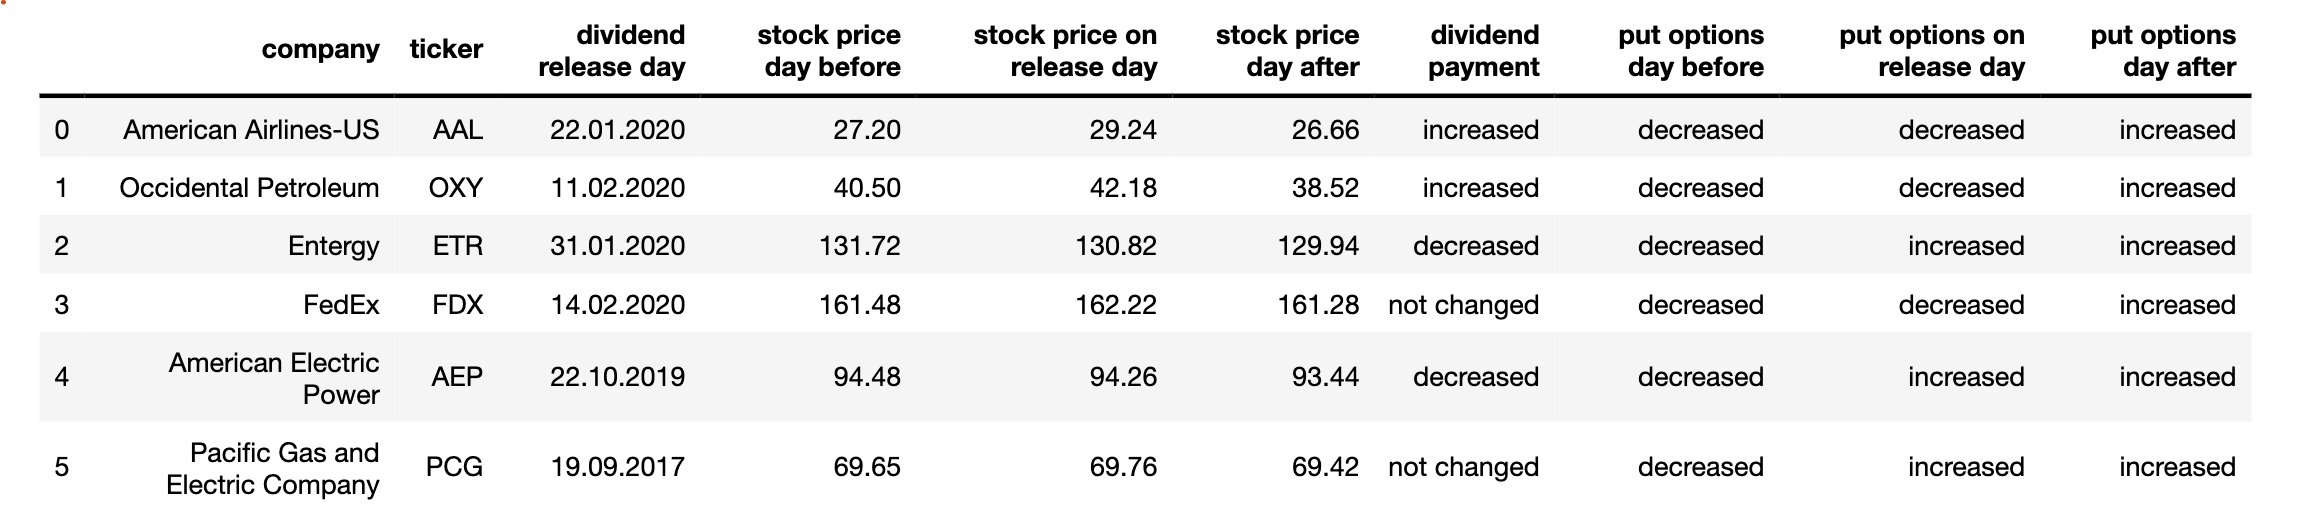
\includegraphics[scale = 0.25]{options_info.png}}
    \caption{Информация об изменениях стоимости опционов в зависимости от дивидендов}
    \label{fig:image}
\end{figure}

\section*{11: Итоги, выводы:}


\section*{12: Спасибо за внимание так сказать}




\end{document}